\chapter{Caracterización Óptica}
\section{Reflectancia Difusa}

En la Figura \ref{fig:reflectancia} se puede observar los espectros de
reflectancia difusa de las muestras \ce{Lu3Al_{5-X}Fe_{x}O12}:\ce{Ce^{3+}}.
Donde el material con x = 0.0 mostró una reflectancia intensa en la región
visible (300-800 nm), que disminuye en la región ultravioleta (200-300 nm).  El
aumento de la
concentración de \ce{Fe^{3+}} generó una disminución progresiva de la
reflectancia en
la región visible, así como un fenómeno de desplazamiento del rojo, esto se
puede atribuir a la reducción de energía de banda \cite{Zhou2017}.\\

\begin{figure}[h]
    \centering%

    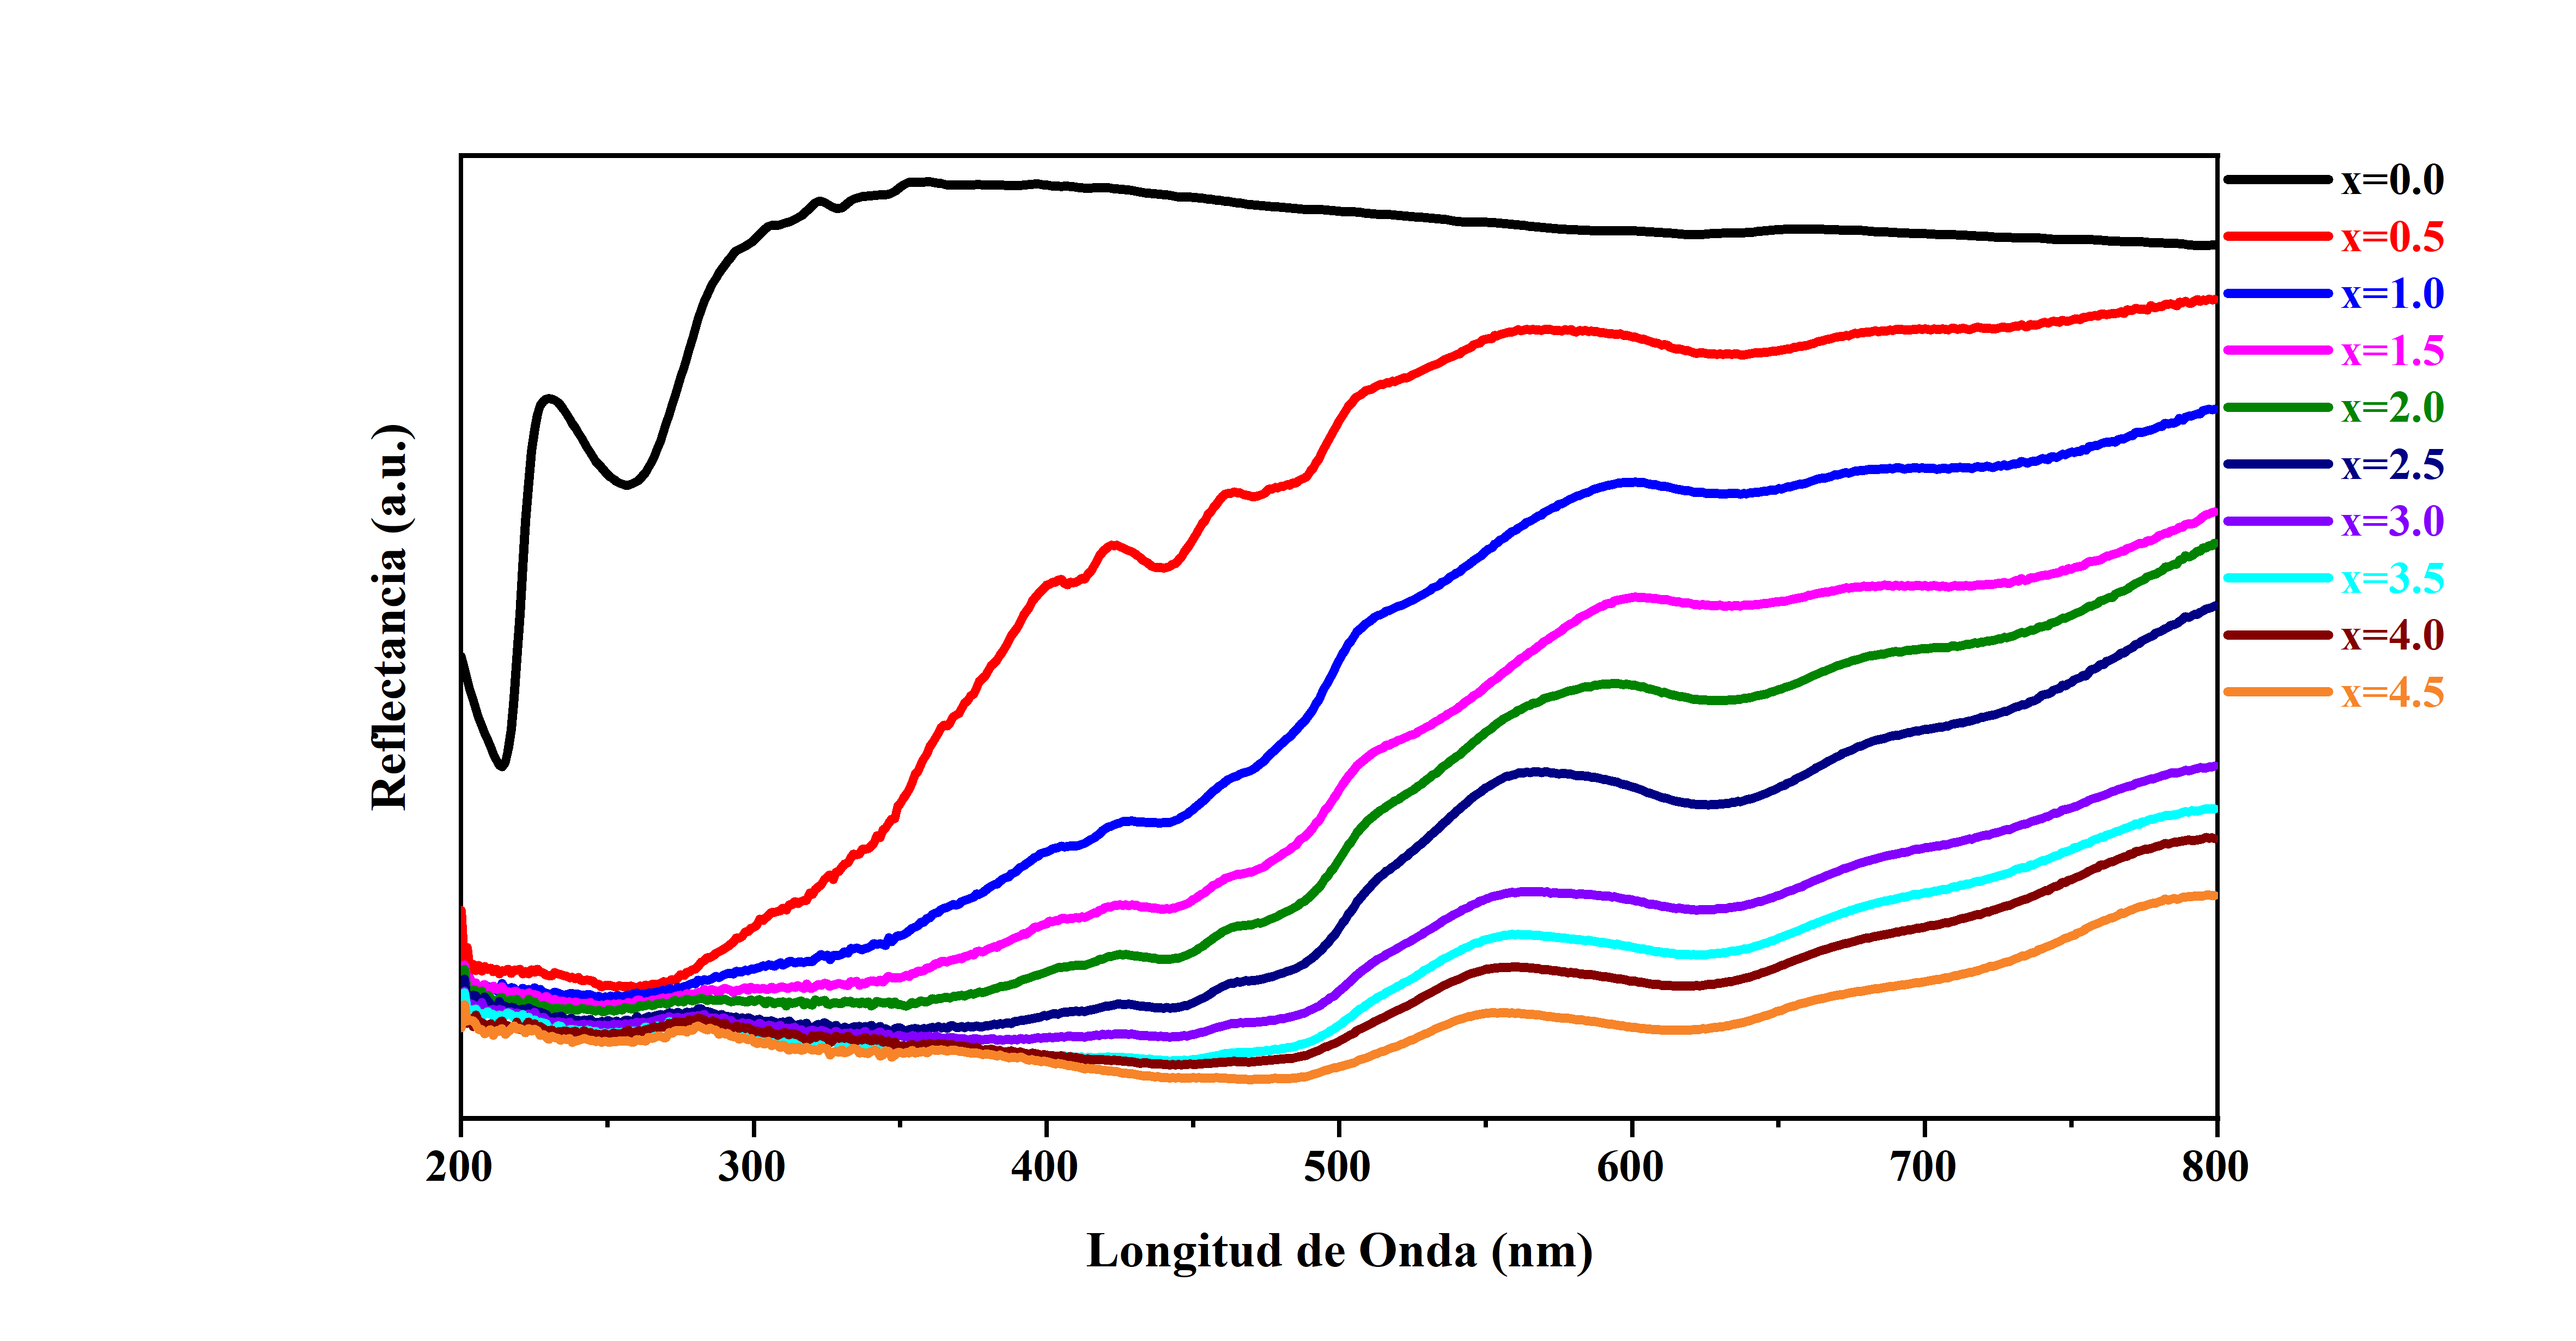
\includegraphics[width=\textwidth]{Kap4/ReflectanciaDifusa.png}%
    \caption{Espectros de reflectancia difusa de las muestras de
    \ce{Lu3Al_{5-X}Fe_{x}O12}:\ce{Ce^{3+}}} \label{fig:reflectancia}
\end{figure}

Los valores de la energía banda prohibida (\ce{E_{g}}) se estimaron mediante
extrapolación
lineal de los diagramas de Tauc \cite{Deng2013}, que se determinaron mediante
la Ecuación \ref{eqn:eq1} \cite{Mott1970}.\\

\begin{equation}
    [(F(R) h \nu)^{n}=A(h \nu - E_{g})]
    \label{eqn:eq1}
\end{equation}

donde,$A$ es una constante proporcional, $h \nu$ es la energía del fotón, $n$
es el coeficiente que denota la naturaleza de la transición ($n=2$ para
transiciones directas permitidas, $n=2/3$ para transiciones directas
prohibidas, $n=1/2$ para transiciones indirectas permitidas y $n=1/3$ para
transiciones indirectas prohibidas) \cite{Mott1970}, y $F(R)$ es la función
Kubeka-Munk
(ver Ecuación \ref{eqn:eq2}) \cite{Simmons1975}, en el que $R$ es la
reflectancia:

\begin{equation}
    F(R)=\frac{(1-R)^2}{2R}
    \label{eqn:eq2}
\end{equation}

En la Figura \ref{fig:tauc} a) y b) se puede observar las gráficas de Tauc para
las
muestras del sistema \ce{Lu3Al_{5-X}Fe_{x}O12}:\ce{Ce^{3+}}. Los datos
experimentales se
ajustaron bien con $n = 2$, lo que indica la existencia de transiciones
directas
permitidas. La $E_{g}$ disminuyó progresivamente conforme al aumento en la
concentración \ce{Fe^{3+}} (ver Figura \ref{fig:tauc} c), lo que se relaciona
con el
incremento del
valor para el parámetro de red \cite{J.C.Inkson2012}. En un semiconductor
cúbico, la $E_{g}$
disminuye proporcionalmente al cuadrado del parámetro de red \cite{Dalven1973},
esto se
puede atribuir a la energía de enlace de la disminución de valencia al aumentar
la distancia interatómica, requiriendo menos energía para liberar los
electrones de la banda de conducción.\\

\begin{figure}[H]
    \centering%

    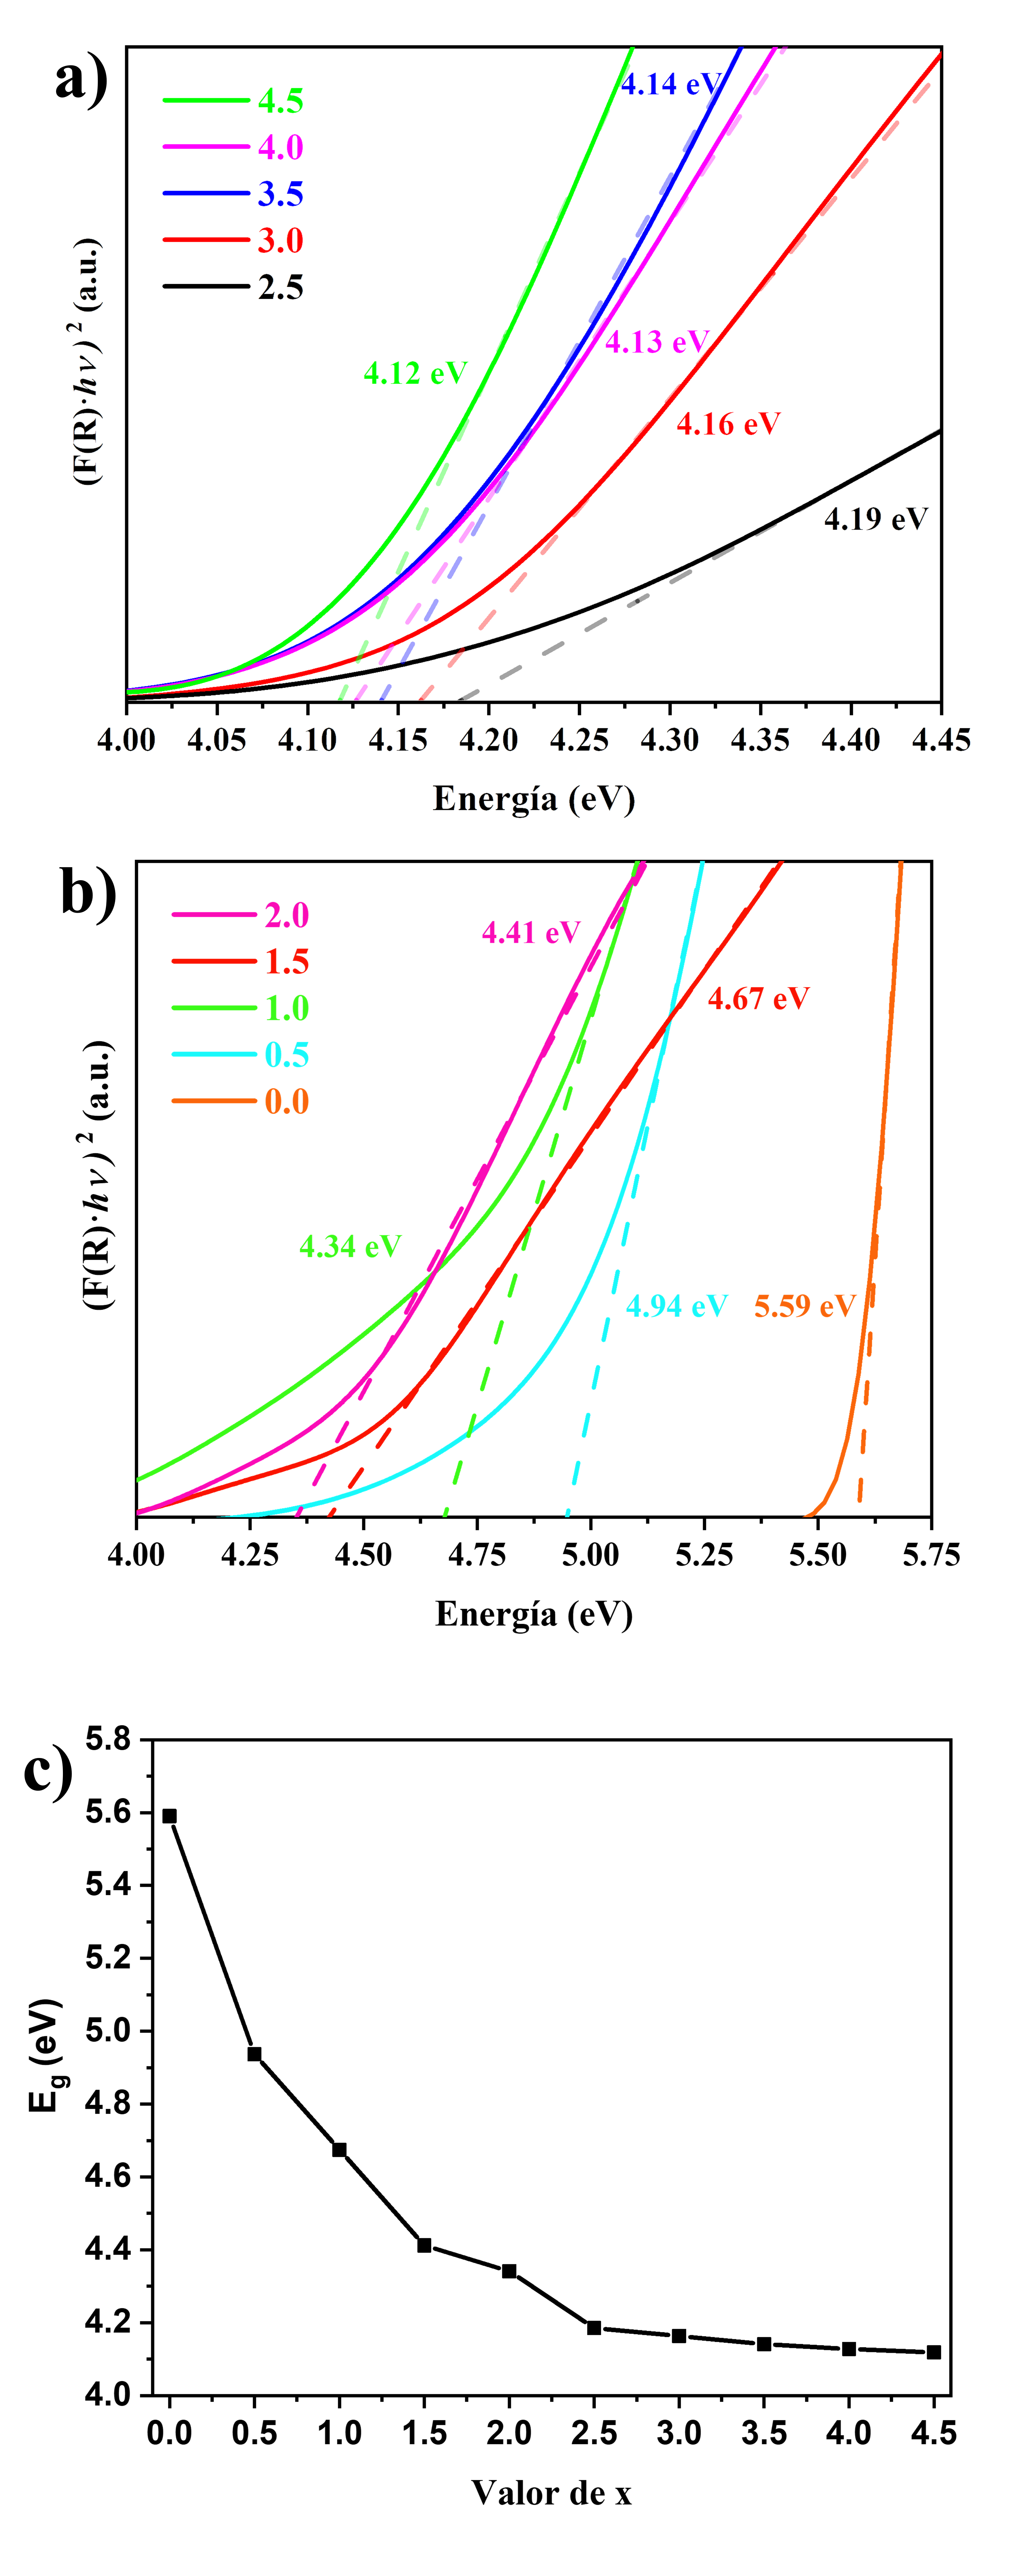
\includegraphics[width=0.45\textwidth]{Kap4/Tauc2.png}%
    \caption{a) y b) Gráficas de Tauc de las muestras del sistema
    \ce{Lu3Al_{5-X}Fe_{x}O12}:\ce{Ce^{3+}} y c) $E_g$ en función de la
    concentración de \ce{Fe^{3+}}}\label{fig:tauc}
\end{figure}

\section{Espectro de Absorción}

En la estructura granate, los cationes \ce{Ce^{3+}} se encuentran en los sitios
dodecaédricos, generando un estado doblemente degenerado ($^{2}E_{g}$) y un
estado
triplemente degenerado ($^{2}T_{g}$), con un campo cristalino habitual que se
divide
($\varepsilon_{0}$) entre el nivel más bajo ($5d_{1}$) y el nivel más alto
($5d_5$). Sin embargo, los
niveles de $5d_1$ y $5d_2$ del estado $^2E_g$ se dividen más que los de
coordinación
cúbica u octaédrica, lo que lleva a una división adicional del campo cristalino
\cite{Dorenbos2003}
($\Delta_{1-2}$). Como resultado, todas las muestras exhibieron tres bandas de
adsorción en la región UV-Vis (Figura \ref{fig:abso}). Las bandas ubicadas en
el rango
espectral de 200-230 nm son atribuibles a las transiciones superpuestas $4f$
$(2F_{5/2}) \rightarrow ^2T_g(^5d_{5,4,3})$ y las bandas restantes ubicadas
alrededor de 350 y 450
nm corresponden a las transiciones $4f(^2F_{5/2}) \rightarrow ^2E_g (^5d_2)$ y
    $4f(^2F_{5/2}) \rightarrow ^2E_g
    (5d_1)$, respectivamente \cite{Ueda2019}.\\

\begin{figure}[H]
    \centering%

    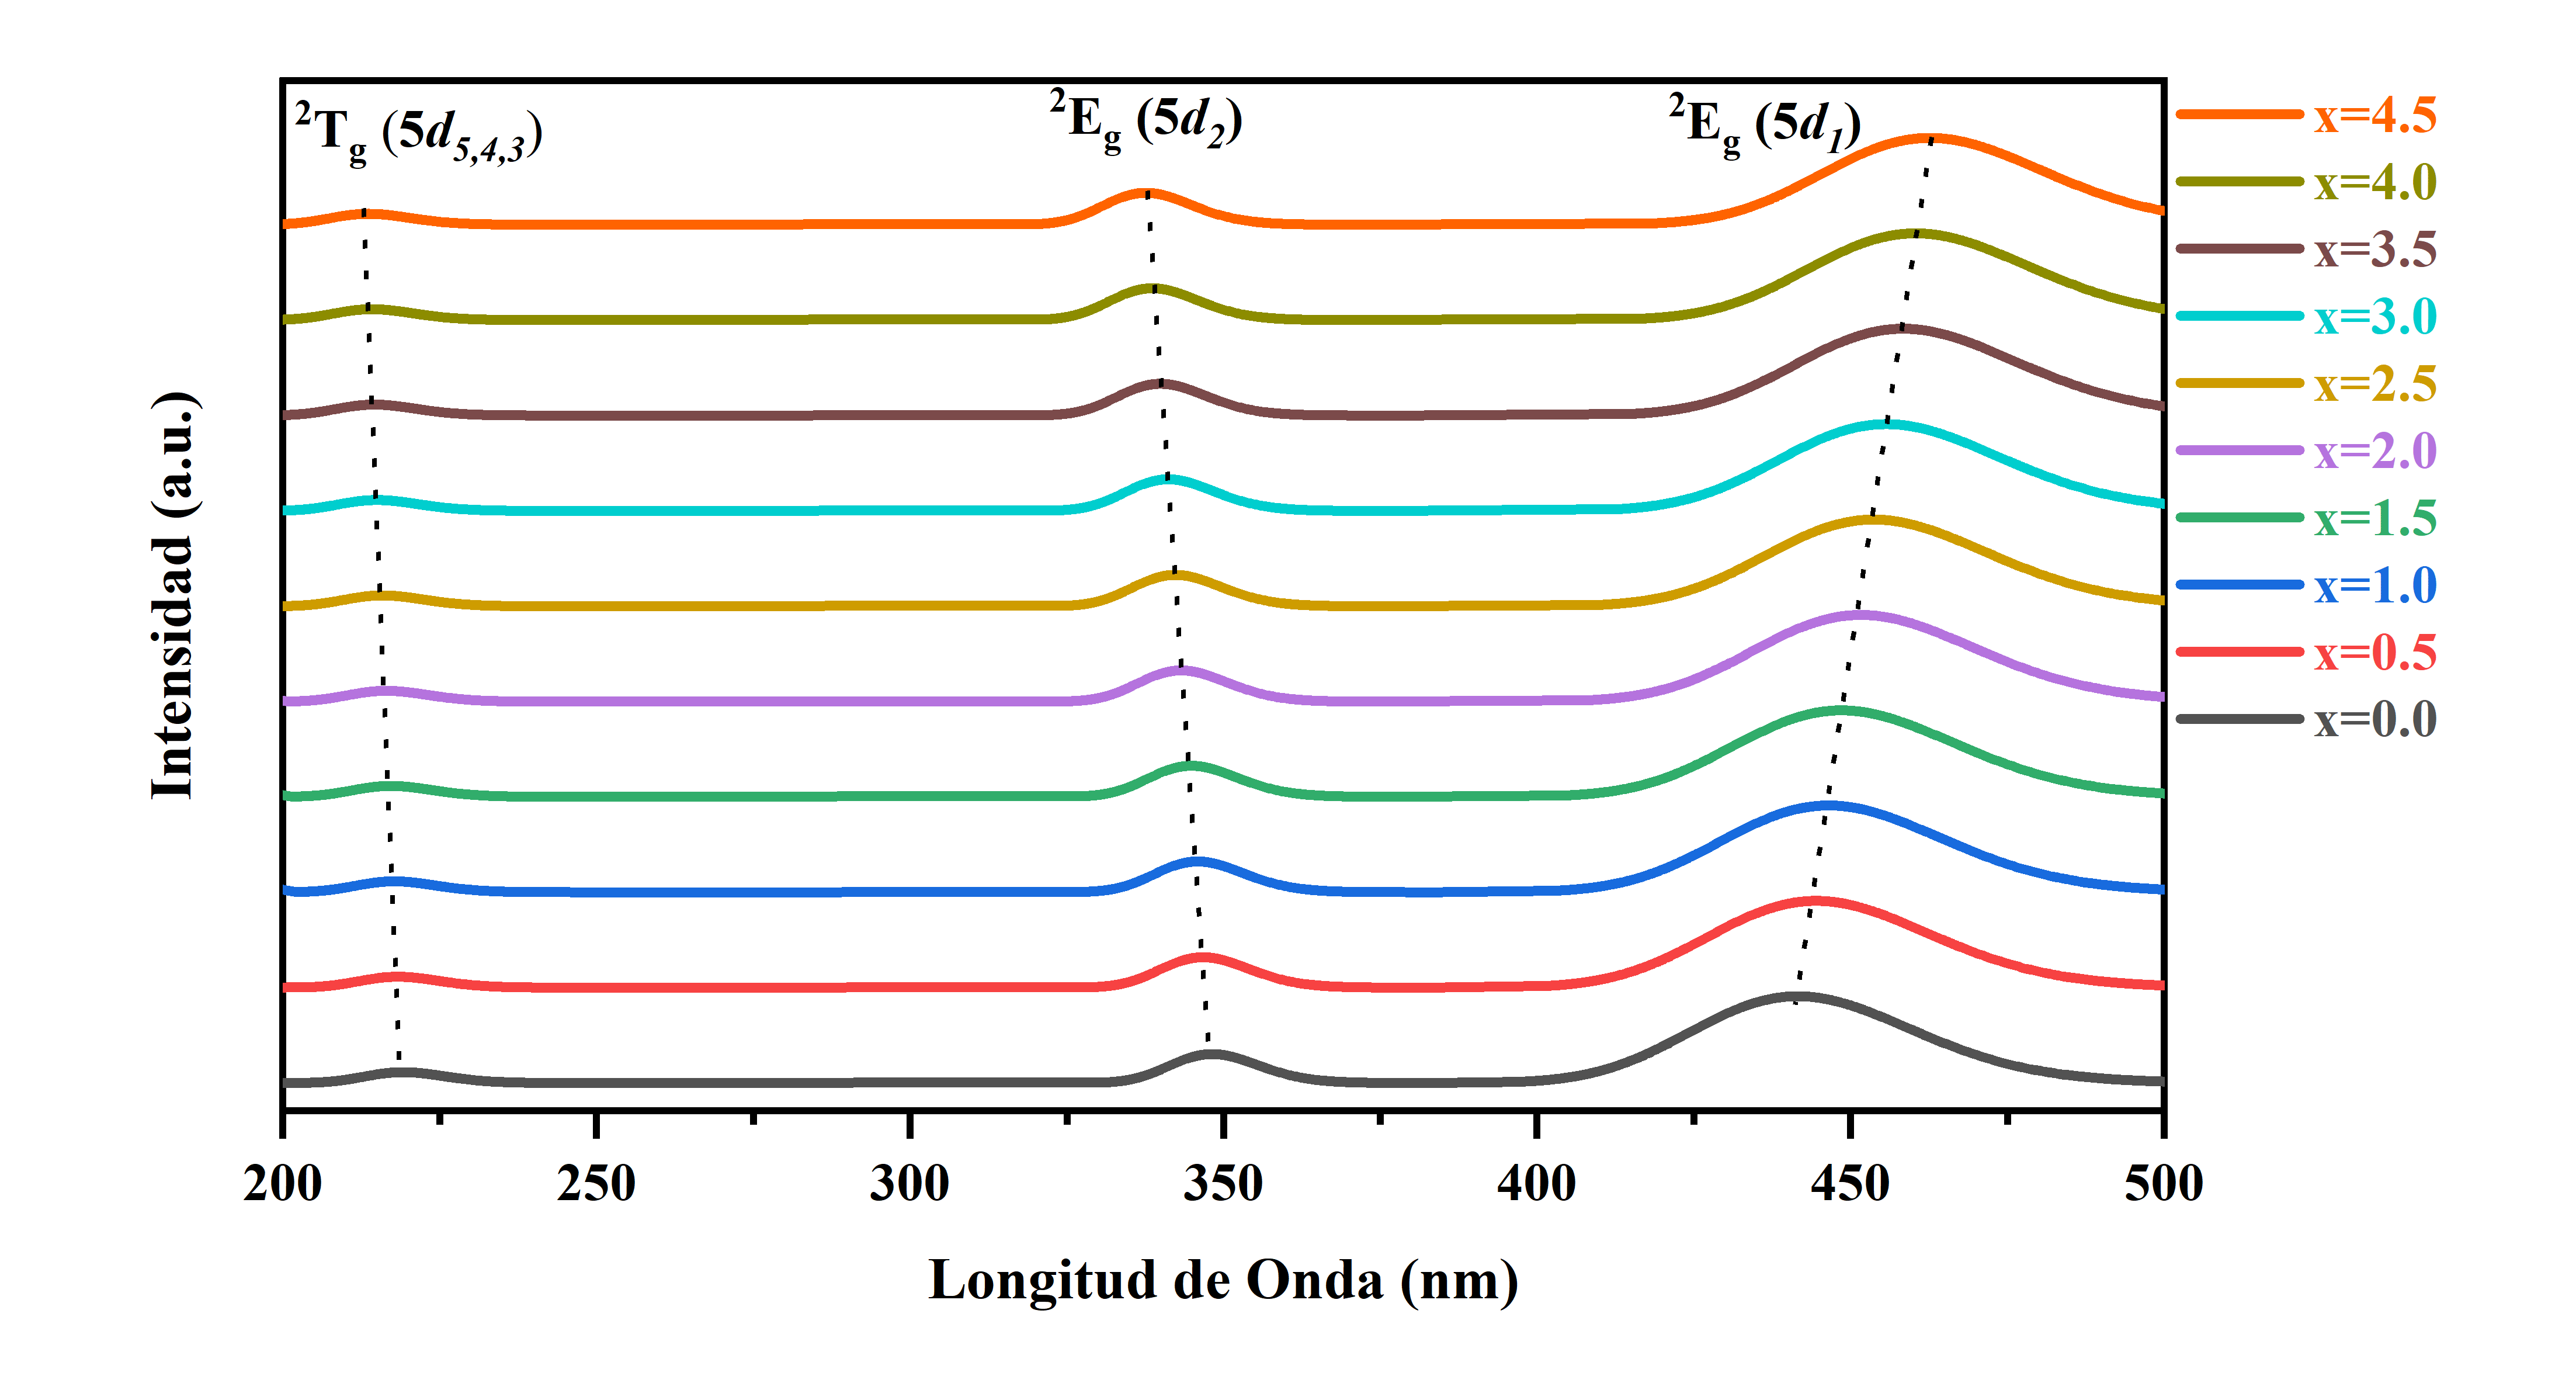
\includegraphics[width=\textwidth]{Kap4/Absorcion.png}%
    \caption{Espectros de absorción en la región UV-Vis para las muestras de
    \ce{Lu3Al_{5-X}Fe_{x}O12}:\ce{Ce^{3+}} (0.0 $\leq x \leq$
    4.5)}\label{fig:abso}
\end{figure}

Al aumentar la concentración de \ce{Fe^{3+}} en las muestras, las bandas
asociadas a
las transiciones $4f(^2F_{5/2}) \rightarrow ^2T_g (5d_{5,4,3})$ y
$4f(^2F_{5/2}) \rightarrow ^2E_g (5d_2)$ mostraron
un desplazamiento hacia longitudes de onda más corta (desplazamiento hacia el
azul). Por el contrario, la banda asociada a la transición $4f(^2F_{5/2})
    \rightarrow ^2E_g(5d_1)$ mostró un desplazamiento hacia longitudes de onda
más
largas
(desplazamiento hacia el rojo). La energía de los niveles $5d$ es sensible
a
las variaciones estructurales \cite{Xu2014}, y la energía de separación del
campo
cristalino \cite{Dorenbos2003}. El dopaje con \ce{Fe^{3+}} generó la
intensificación de las
energías
($\varepsilon_{0}$) y $\Delta_{1-2}$, aumentando la energía de las
$^2T_g(5d_{5,4,3})$ y los niveles $2E_g(5d_2)$,
pero disminuyendo la energía del nivel $2E_g(5d_1)$. La longitud de onda de las
bandas de absorción y los valores de las energías ($\varepsilon_{0}$) y
$\Delta_{1-2}$ se presentan en la
Tabla \ref{tab:longitudOnda}. Con base en cálculos teóricos, realizados por
Chen et al
\cite{Chen2015a}. Se
estableció que la inserción de cationes más grandes en la estructura del
granate genera un fuerte efecto compresivo, lo que lleva a la generación de
orbitales moleculares híbridos a partir del orbitales d del metal y el orbital
2p del oxígeno.\\

\begin{table}[h]
    \caption{Longitud de onda (nm) y energía (eV) de los estados excitados para
    \ce{Ce^{3+}} en materiales \ce{Lu3Al_{5-X}Fe_{x}O12}:\ce{Ce^{3+}}, y
    energías
    de separación de campo cristalino $\varepsilon_0$ y $\Delta_{1-2}$}
    \label{tab:longitudOnda}
    \resizebox{\textwidth}{!}{%
        \begin{tabular}{@{}llllllll@{}}
            \toprule
                                                  & \multicolumn{5}{l}{Banda de
                Absorción nm (eV)}

                                                  &
                                                  &
            \\ \cmidrule(lr){2-6}
            \multirow{-2}{*}{Valor de X}          & 5d5
                                                  & 5d4
                                                  & 5d3
                                                  & 5d2
                                                  & 5d1
                                                  &
            \multirow{-2}{*}{$\varepsilon (eV)$}                   & \multirow{-2}{*}{$\Delta_{1-2}$
                (eV)}
            \\ \midrule
            0.0                                   & 209 (5.93)
                                                  & 219
            (5.66)                             & 228 (5.44)
                                                  & 348
            (3.56)                             & 442 (2.81)
                                                  &
            2.63                                  & 0.75
            \\
            0.5                                   & 208
            (5.95)                             &
            218 (5.68) & 227
            (5.46)                             &
            347 (3.58) & 444
            (2.79)                             &
            2.67          &
            0.79
            \\
            1.0                                   & 208 (5.97)
                                                  & 218
            (5.69)                             & 227 (5.47)
                                                  & 346
            (3.59)                             & 446 (2.78)
                                                  &
            2.69                                  & 0.81
            \\
            1.5                                   & 207
            (5.99)                             &
            217 (5.71) & 226
            (5.48)                             &
            345 (3.60) & 448
            (2.76)                             &
            2.72          &
            0.83
            \\
            2.0                                   & 206 (6.01)
                                                  & 216
            (5.73)                             & 225 (5.50)
                                                  & 343
            (3.61)                             & 452 (2.75)
                                                  &
            2.75                                  & 0.87
            \\
            2.5                                   & 206
            (6.02)                             &
            216 (5.74) & 225
            (5.51)                             &
            342 (3.62) & 454
            (2.73)                             &
            2.78          &
            0.89
            \\
            3.0                                   & 205 (6.05)
                                                  & 215
            (5.77)                             & 224 (5.53)
                                                  & 341
            (3.63)                             & 456 (2.72)
                                                  &
            2.81                                  & 0.91
            \\
            3.5                                   & 205
            (6.06)                             &
            215 (5.78) & 224
            (5.54)                             &
            340 (3.65) & 458
            (2.71)                             &
            2.84          &
            0.94
            \\
            4.0                                   & 204 (6.07)
                                                  & 214
            (5.79)                             & 223 (5.56)
                                                  & 339
            (3.66)                             & 460 (2.69)
                                                  &
            2.86                                  & 0.97
            \\
            4.5                                   & 204
            (6.09)                             &
            214 (5.80) & 223
            (5.57)                             &
            338 (3.67) & 462
            (2.68)                             &
            2.89          &
            0.99
            \\ \bottomrule
        \end{tabular}%
    }
\end{table}

Esta hibridación de orbitales conduce a una fuerte disminución de la energía de
banda prohibida ($E_g$) debido a la expansión de la banda de conducción, la
reducción de la masa efectiva del electrón y una intensificación de la energía
del campo cristalino \cite{Chen2015a}.\\

\section{Fotoluminisencia}

Las muestras de \ce{Lu3Al_{5-X}Fe_{x}O12}:\ce{Ce^{3+}} con x $\geq $ 1.5
exhibieron fotoluminiscencia
bajo irradiación azul (436 nm), exhibiendo bandas asimétricas en el rango
espectral de 450–650 nm (Figura \ref{fig:foto} a). Las bandas de emisión fueron
decombolucionadas en dos perfiles gaussianos (como se muestra en el inserto de
la Figura \ref{fig:foto} a. las cuales son atribuidas a transiciones desde el
nivel más
bajo de $^2E_g(5d_1)$ a los estados fundamentales $^2F_{5/2}$ y $^2F_{7/2}$,
respectivamente \cite{Yu2014}. Los anchos de banda obtenidos fueron
considerablemente amplios debido
al
fuerte acoplamiento fonónico \cite{Ueda2019}, e indican efectos de campo
cristalino en los
estados excitados del \ce{Ce^{3+}} \cite{Miniscalco1978}. Además, la inserción
de \ce{Fe^{3+}}
provocó un
desplazamiento de las bandas de emisión, lo que sugiere que las bandas se deben
a una transferencia de carga no relajada entre los cationes \ce{Ce^{3+}}
\cite{Zhang2014}.\\

\begin{figure}[h]
    \centering%

    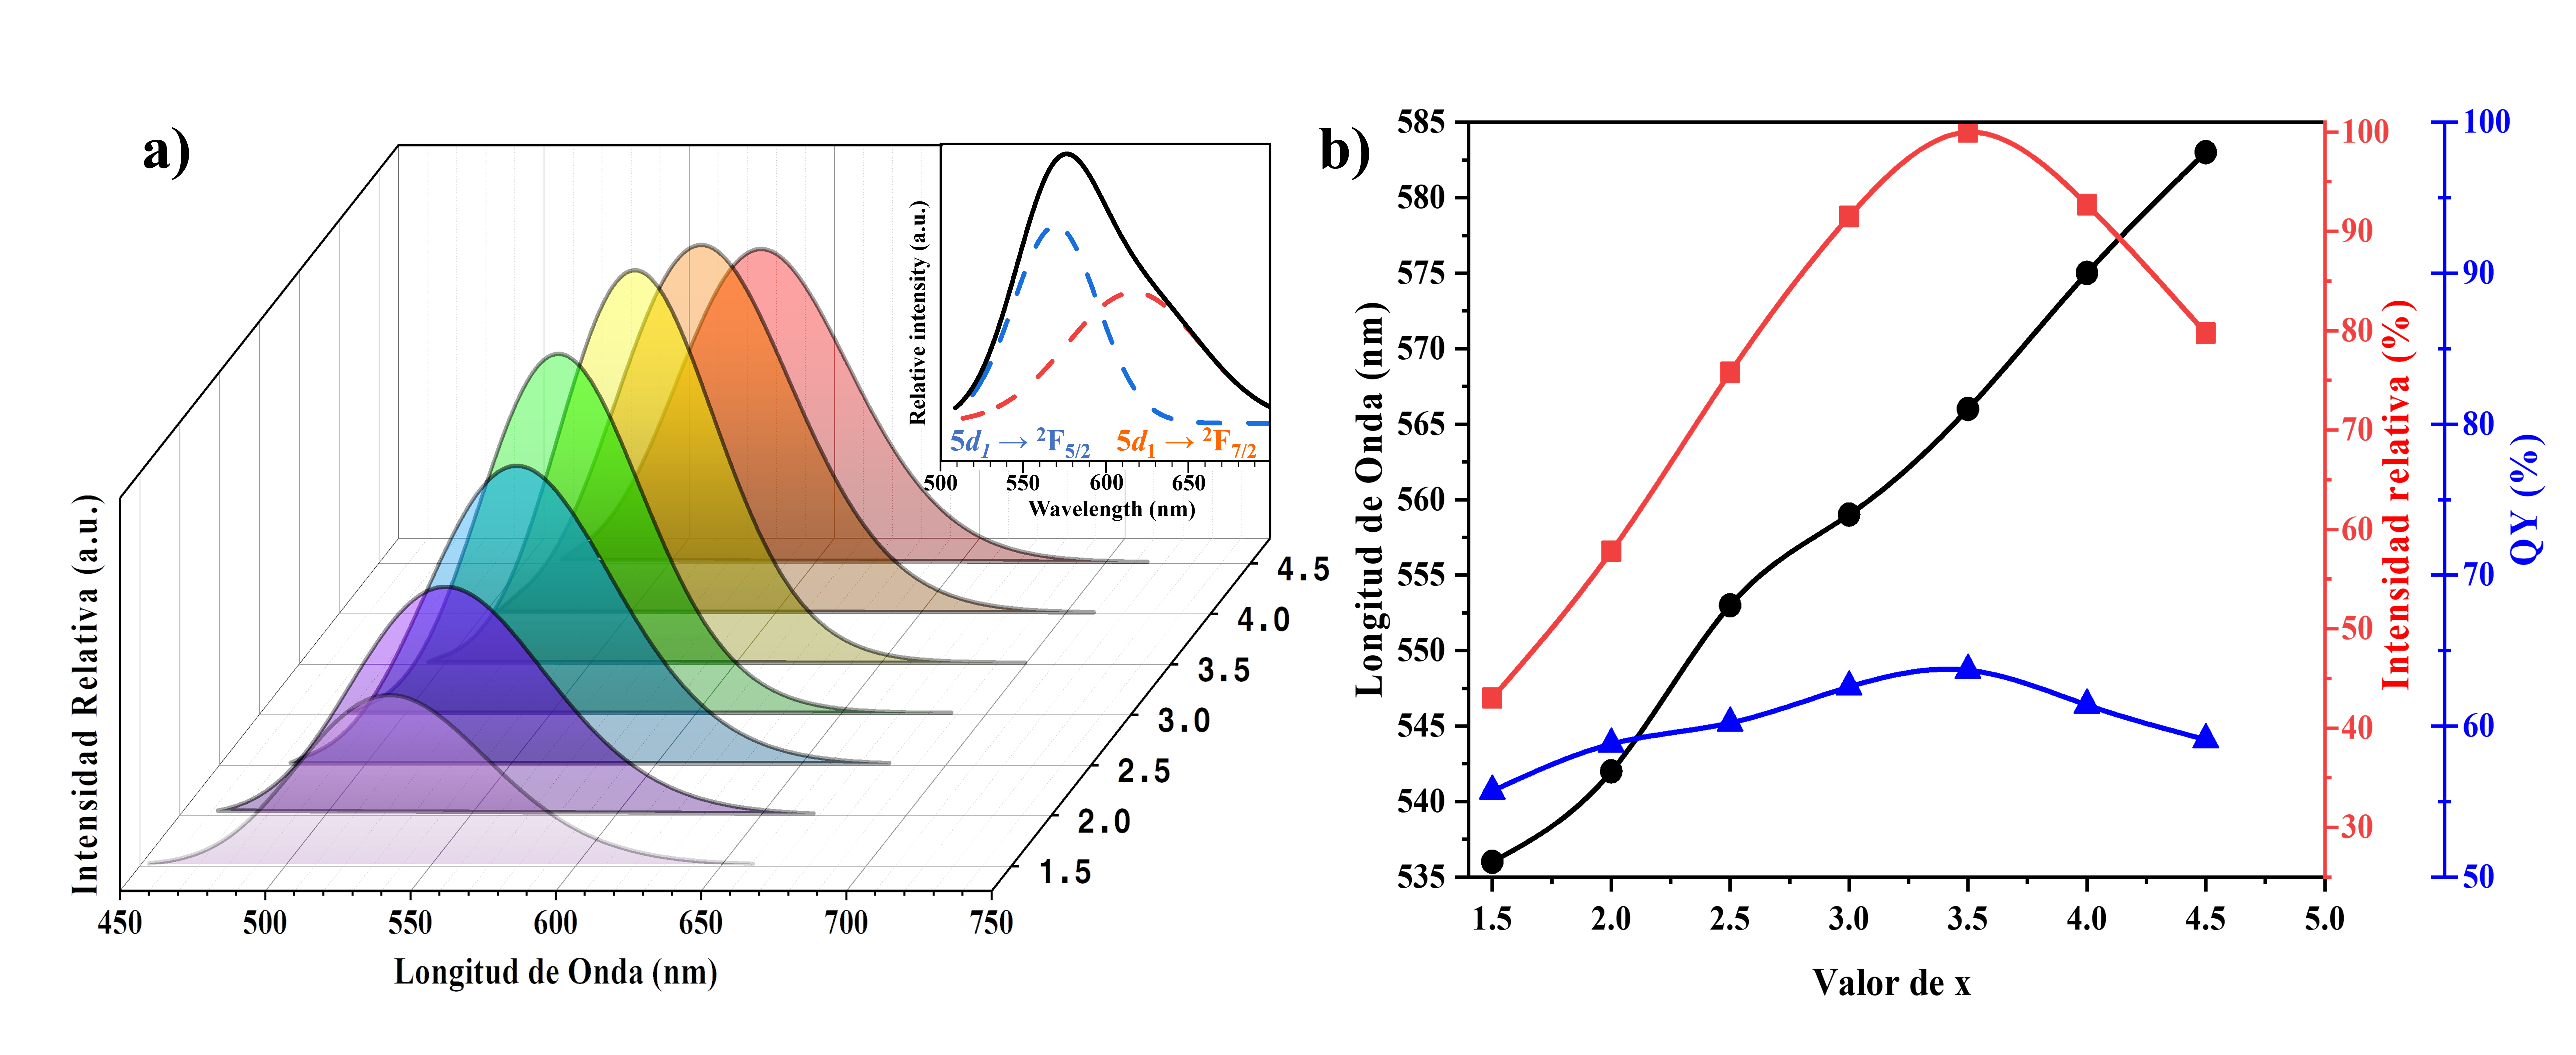
\includegraphics[width=\textwidth]{Kap4/Fotoluminisencia.png}%
    \caption{Espectros de fotoluminiscencia bajo excitación de 436 nm de las
    muestras \ce{Lu3Al_{5-X}Fe_{x}O12}:\ce{Ce^{3+}} con 1.5 $\leq x \leq  $ 4.5
    (a). Longitud de onda, intensidad de emisión y rendimiento cuántico de la
    banda
    de emisión en función del valor x (b). perfiles gaussianos atribuidos a las
    transiciones más bajas de $^2E_g(5d_1)\rightarrow ^2F_{5/2}$ y $^2E_g(5d_1)
        \rightarrow ^2F_{7/2}$ de \ce{Ce^{3+}}}\label{fig:foto}
\end{figure}

Se observó un ligero desplazamiento hacia el rojo al aumentar la concentración
de \ce{Fe^{3+}} (Figura \ref{fig:foto} b), que se atribuye a la energía
$\Delta_{1-2}$
intensificada,
generando una menor separación entre el nivel más bajo de $^2E_g(5d_1)$ y los
estados fundamentales $4f(^2F_{5/2}$ y $^2F_{7/2})$ \cite{Chen2015a,Hu2019}.
Como se
informó
anteriormente, la inserción de \ce{Fe^{3+}} condujo a la expansión de la celda
unidad
y, por lo tanto, se esperarían fenómenos de desplazamiento hacia el azul
\cite{Ueda2019,Dorenbos2013}, y se ajusta a los resultados presentados en
trabajos de
investigación
similares, en los que se insertan cationes más grandes en las estructuras del
granate huésped \cite{Chen2015a,Kamada2011,Hu2015}. Además de la energía
$\Delta_{1-2}$
intensificada, el
desplazamiento al rojo de los espectros de emisión puede atribuirse al aumento
del desplazamiento de Stokes (SS) dentro de los estados fundamentales y el
estado excitado más bajo ($5d_1$). La energía de desplazamiento de Stokes es
proporcional al grado de interacción electrón-fonón \cite{Ueda2019}. Entonces,
la
interacción electrón-fonónica se haría más fuerte al aumentar la concentración
de \ce{Fe^{3+}}, lo que conduciría a un aumento en el desplazamiento de Stokes.
La
banda de emisión de los materiales y los valores del desplazamiento de Stokes
se presentan en la Tabla \ref{tab:emision}.\\

\begin{table}[]
    \caption{Banda de emisión y desplazamiento de Stokes de \ce{Lu3Al_{5-X}Fe_{x}O12}:\ce{Ce^{3+}}}
    \label{tab:emision}
    \resizebox{\textwidth}{!}{%
        \begin{tabular}{cccc}
            \hline
            Valor de x & Banda de Emisión (nm) & Desplazamiento de Stokes (nm)
                       &
            Desplazamiento de Stokes (eV)
            \\ \hline
            
            1.5       & 536 (2.31)         & 88
                       & 0.45
            \\
            2.0       & 542 (2.29)         & 90
                       & 0.46
            \\
            
            2.5       & 553 (2.24)         & 99
                       & 0.49
            \\
            3.0       & 559 (2.22)         & 103
                       & 0.50
            \\
            
            3.5       & 566 (2.19)         & 108
                       & 0.51
            \\
            4.0       & 575 (2.16)         & 115
                       & 0.54
            \\
            
            4.5       & 583 (2.13)         & 120
                       & 0.55
            \\ \hline
        \end{tabular}%
    }
\end{table}

Para aplicaciones de w-LED, el rendimiento cuántico (QY) es un parámetro
importante en la evaluación de fósforos empleados para fabricación de w-LED. El
QY se midió por debajo de 436 nm y se calculó usando la ecuación
\ref{eqn:eq3} \cite{Liu2013}.\\

\begin{equation}
    \eta_{QY} =\frac{\int L_s}{\int E_R-\int E_s}
    \label{eqn:eq3}
\end{equation}

Donde $L_s$ es el espectro de emisión de la muestra, $E_s$ y $E_R$ representan
la luz de excitación con y sin la muestra en la esfera integradora,
respectivamente. El
valor para $\eta_{QY}$ de los materiales aumentó progresivamente, alcanzando un
máximo del 64\% para el material con x = 0.35 (Figura 82 b). Aunque los valores
de
$\eta_{QY}$ no son tan altos como los del granate comercial
\ce{Y3Al5O12}:\ce{Ce^{3+}},
son más altos que los reportados en otros estudios y podría mejorarse ajustando
las
propiedades estructurales y morfológicas. El aumento de la concentración de
\ce{Fe^{3+}} también generó una mayor intensidad de emisión debido a la
absorción
mejorada a 436 nm (Figura \ref{fig:foto} b), alcanzando un máximo cuando x =
3.5.\\

Los valores máximos de $\eta_{QY}$ y de intensidad de emisión cuando x = 3.5
pueden atribuirse a modos de fonón inaccesibles debido a la inserción de un
sustituyente grande como \ce{Fe^{3+}} en la estructura rígida
\cite{George2013}. (x = 4.0 y
4.5) se deben al hecho de que la inserción de \ce{Fe^{3+}} en la estructura
anfitrión generó la expansión del parámetro de red, aumentando la probabilidad
de transferencia
no radiativa entre cationes \ce{Ce^{3+}} \cite{Chen2015a}. La distancia crítica
($R_c$)
entre cationes \ce{Ce^{3+}} determina cuál mecanismo es responsable de la
extinción, el valor
de ($R_c$) se estimó utilizando la siguiente ecuación \cite{Blasse1968}:\\

\begin{equation}
    R_c \approx 2\left(\frac{3V}{4 \pi X_c N}\right)^{-3}
    \label{eqn:eq4}
\end{equation}

Donde $V$ es el volumen de celda unitaria de la red del anfirión
($V=1797.57$\r{A}$^3$), $N$ es el número de sitios dopantes disponibles en la
celda
unitaria ($N=24$) y $X_c$ es la concentración de cationes \ce{Ce^{3+}}
($X_c=0.045$). El
valor de $R_c$ fue de $14.70$ \r{A} aproximadamente, lo que implica que la
extinción de la
concentración se debe a la interacción eléctrica multipolar
\cite{Li2018,Hua2016}.\\

Las coordenadas de cromaticidad CIE se determinaron a partir de los espectros
de emisión de las muestras y se calculó la pureza del color usando la siguiente
ecuación \cite{KaviRasu2017}:\\

\begin{equation}
    PurezaColor = \sqrt{\frac{(x-x_n)^2+(y-y_n)^2}{(x_i-x_n)^2+(y_i-y_n)^2}}
    \times 100\%
    \label{eqn:eq5}
\end{equation}

Donde ($x$, $y$) son las coordenadas de cromaticidad CIE, ($x_n$, $y_n$) se
refiere a las coordenadas de cromaticidad CIE para el color blanco y ($x_i$,
$y_i$) son las
coordenadas de la longitud de onda dominante.\\

La Tabla \ref{tab:croma} enumera las coordenadas de cromaticidad CIE
y la pureza del color bajo excitación de 436 nm para los materiales
\ce{Lu3Al_{5-X}Fe_{x}O12}:\ce{Ce^{3+}}. Se pudo observar que el dopaje con
\ce{Fe^{3+}} permite aumentar
la pureza del color hasta un 95,2\% (x = 4.5).\\

\begin{table}[]
    \centering
    \caption{Coordenadas cromáticas CIE y pureza color para las muestras \ce{Lu3Al_{5-X}Fe_{x}O12}:\ce{Ce^{3+}} $(1.5\leq x\leq 4.5)$}
    \label{tab:croma}
    \begin{tabular}{llll}
    \hline
         & \multicolumn{2}{l}{Coordenadas CIE} &       \\ \cline{2-3}
    \multirow{-2}{*}{Valor de x} & x & y & \multirow{-2}{*}{Pureza del Color} \\ \hline
    0.15 & 0.3112           & 0.6002           & 77.7\% \\
     
    0.20 & 0.3504           & 0.5917           & 82.3\% \\
    0.25 & 0.3893           & 0.5710           & 88.1\% \\
     
    0.30 & 0.4201           & 0.5508           & 93.1\% \\
    0.35 & 0.4291           & 0.5504           & 93.1\% \\
     
    0.40 & 0.4612           & 0.5321           & 94.8\% \\
    0.45 & 0.4817           & 0.510            & 95.2\% \\ \hline
    \end{tabular}
    \end{table}

Por otro lado, el diagrama de cromaticidad CIE presentado en la Figura
\ref{fig:croma}
muestra que la emisión se ajustó de verde a naranja por el dopaje \ce{Fe^{3+}}
en los
granates.\\

\begin{figure}[t!]
    \centering%

    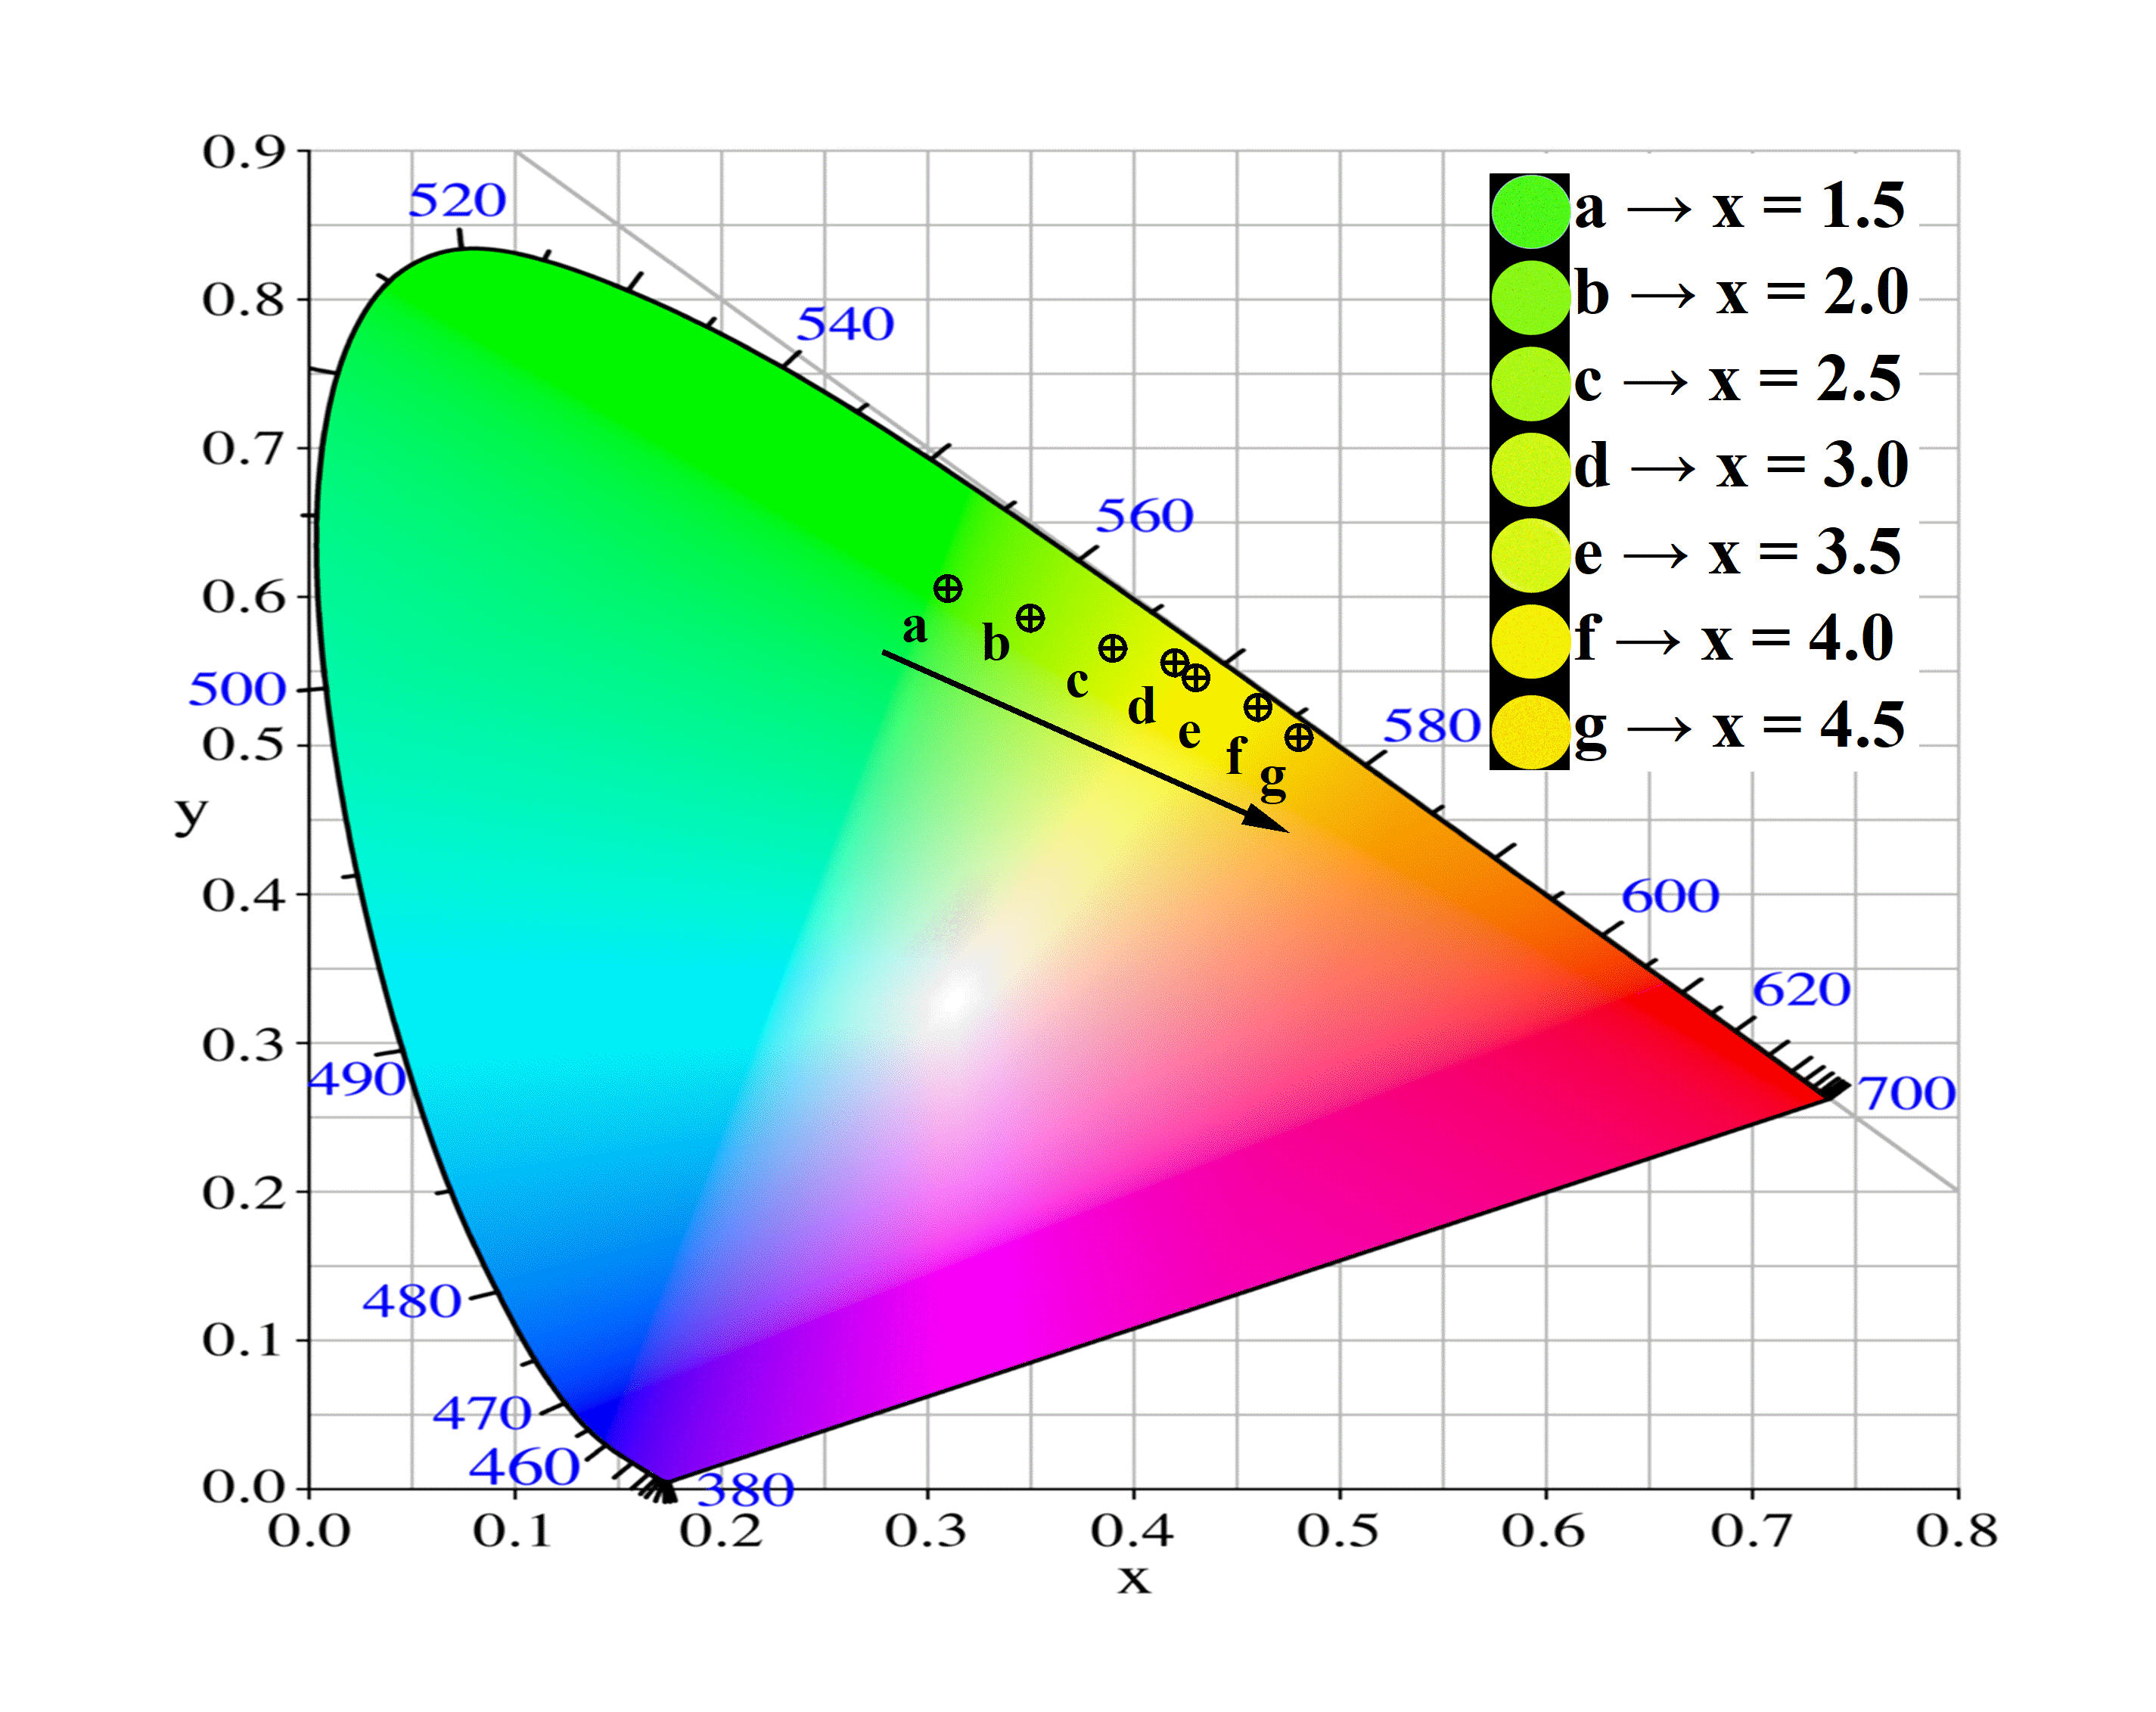
\includegraphics[width=\textwidth]{Kap4/Cromaticidad.png}%
    \caption{Diagrama de cromaticidad CIE para las muestras de
    \ce{Lu3Al_{5-X}Fe_{x}O12}:\ce{Ce^{3+}}	$(1.5\leq x\leq
        4.5)$}\label{fig:croma}
\end{figure}

Los materiales obtenidos exhibieron una gran conversión de color y una alta
pureza de color bajo radiación de luz azul, demostrando sus potenciales
aplicaciones en w-LED. Además, según el análisis óptico, la Figura
\ref{fig:niveles}
muestra
una representación esquemática del efecto
del dopaje con \ce{Fe^{3+}} sobre los niveles de energía de \ce{Ce^{3+}} en los
granates
\ce{Lu3Al_{5-X}Fe_{x}O12}:\ce{Ce^{3+}}.\\

\begin{figure}[h]
    \centering%

    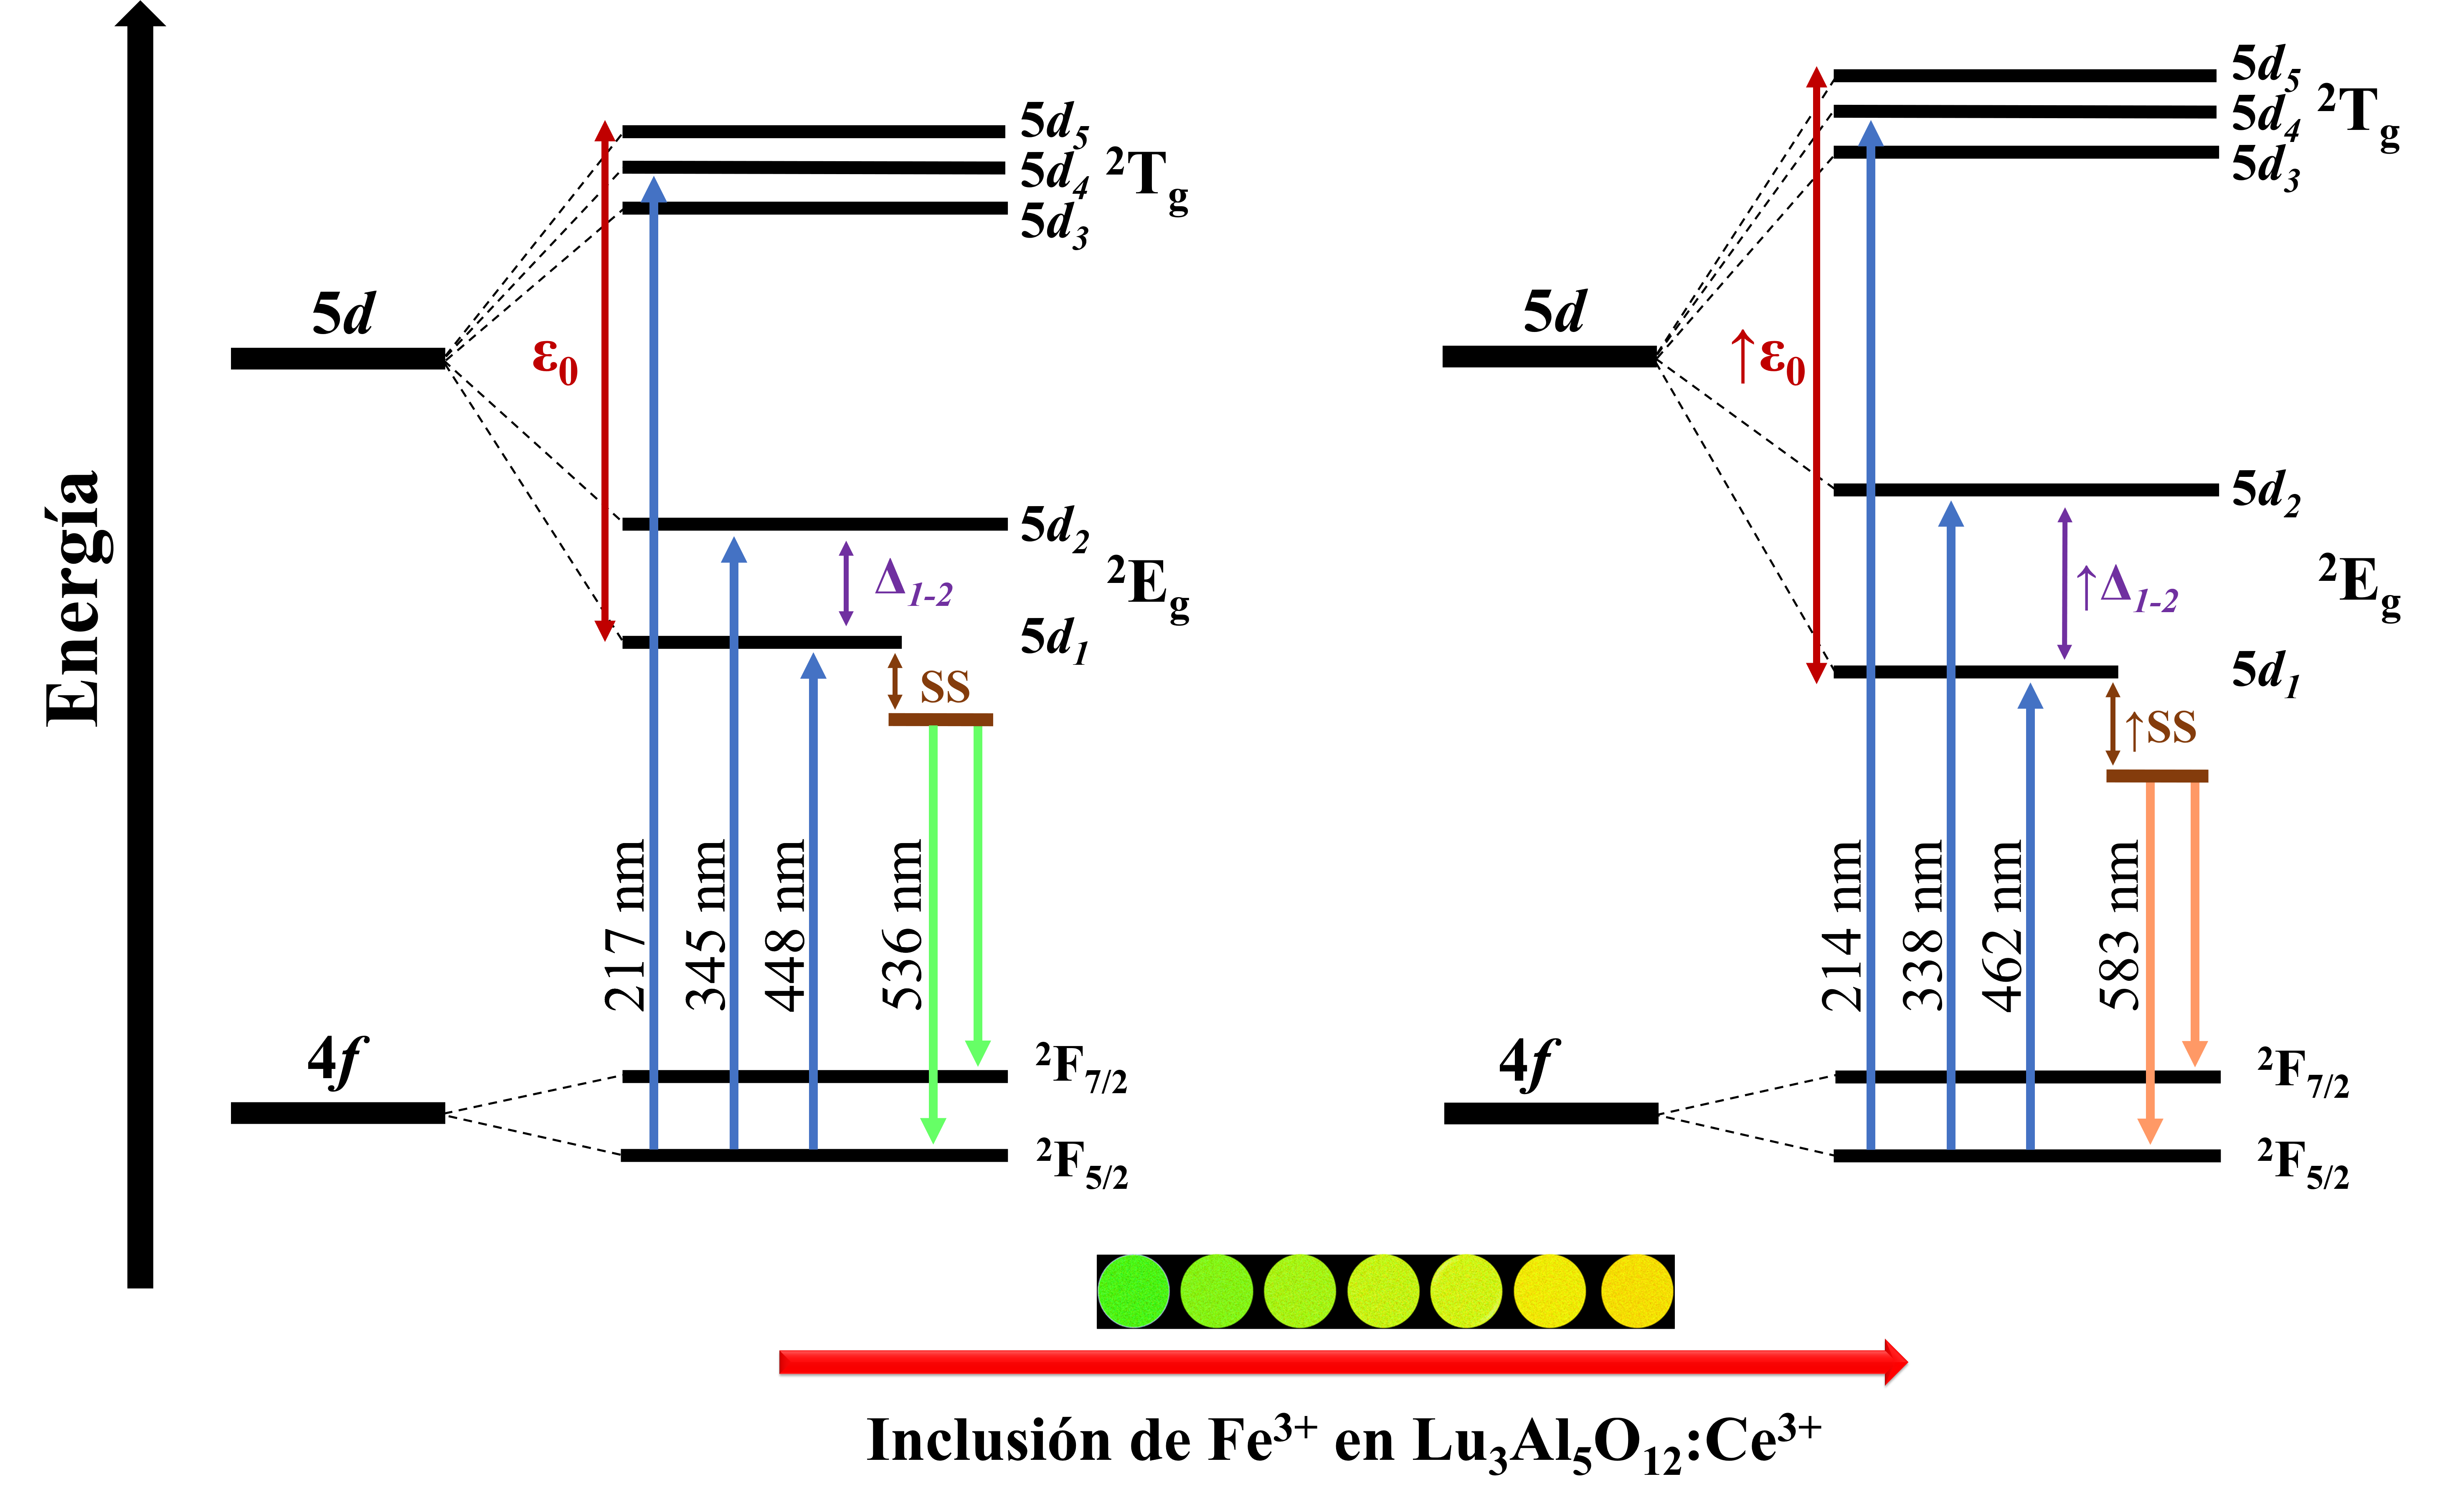
\includegraphics[width=\textwidth]{Kap4/NivelesEnergia.png}%
    \caption{Efecto de la sustitución de \ce{Fe^{3+}} por \ce{Al^{3+}} sobre
    los niveles de energía de \ce{Ce^{3+}} en los granates
    \ce{Lu3Al_{5-X}Fe_{x}O12}:\ce{Ce^{3+}}}\label{fig:niveles}
\end{figure}

Relación entre Temperatura y Fotoluminiscencia. Al trabajar con w-LED, la capa
de fósforo puede alcanzar temperaturas de hasta 150$^{\circ}$C. Entonces, la
estabilidad térmica del fósforo es el parámetro más importante para evaluar su
desempeño para aplicaciones w-LED, especialmente aquellos que emplean en su
fabricación chips que emiten luz azul. Los espectros de fotoluminiscencia en
función de la temperatura para el fósforo
\ce{Lu3Al_{5-X}Fe_{x}O12}:\ce{Ce^{3+}} (para x = 3.5)
bajo una excitación de 436 nm se presentan en la Figura \ref{fig:fotoTemp} a)
La intensidad de
emisión disminuyó gradualmente de 25 a 200$^{\circ}$C debido a los fenómenos de
apagamiento (ver gráfico anexo a Figura \ref{fig:fotoTemp} a). A 150$^{\circ}$C, la
intensidad de
emisión fue del 82,36\% de la intensidad inicial, lo que sugiere un rendimiento
prometedor en el rango de temperatura de funcionamiento de los w-LED. Por otro
lado, la longitud de onda se mantuvo casi sin cambios, lo que demuestra la alta
estabilidad de la emisión de color. El ligero desplazamiento hacia el azul es
atribuible a la excitación asistida por fonones activada térmicamente
\cite{Xia2011}\\

\begin{figure}[h]
    \centering%

    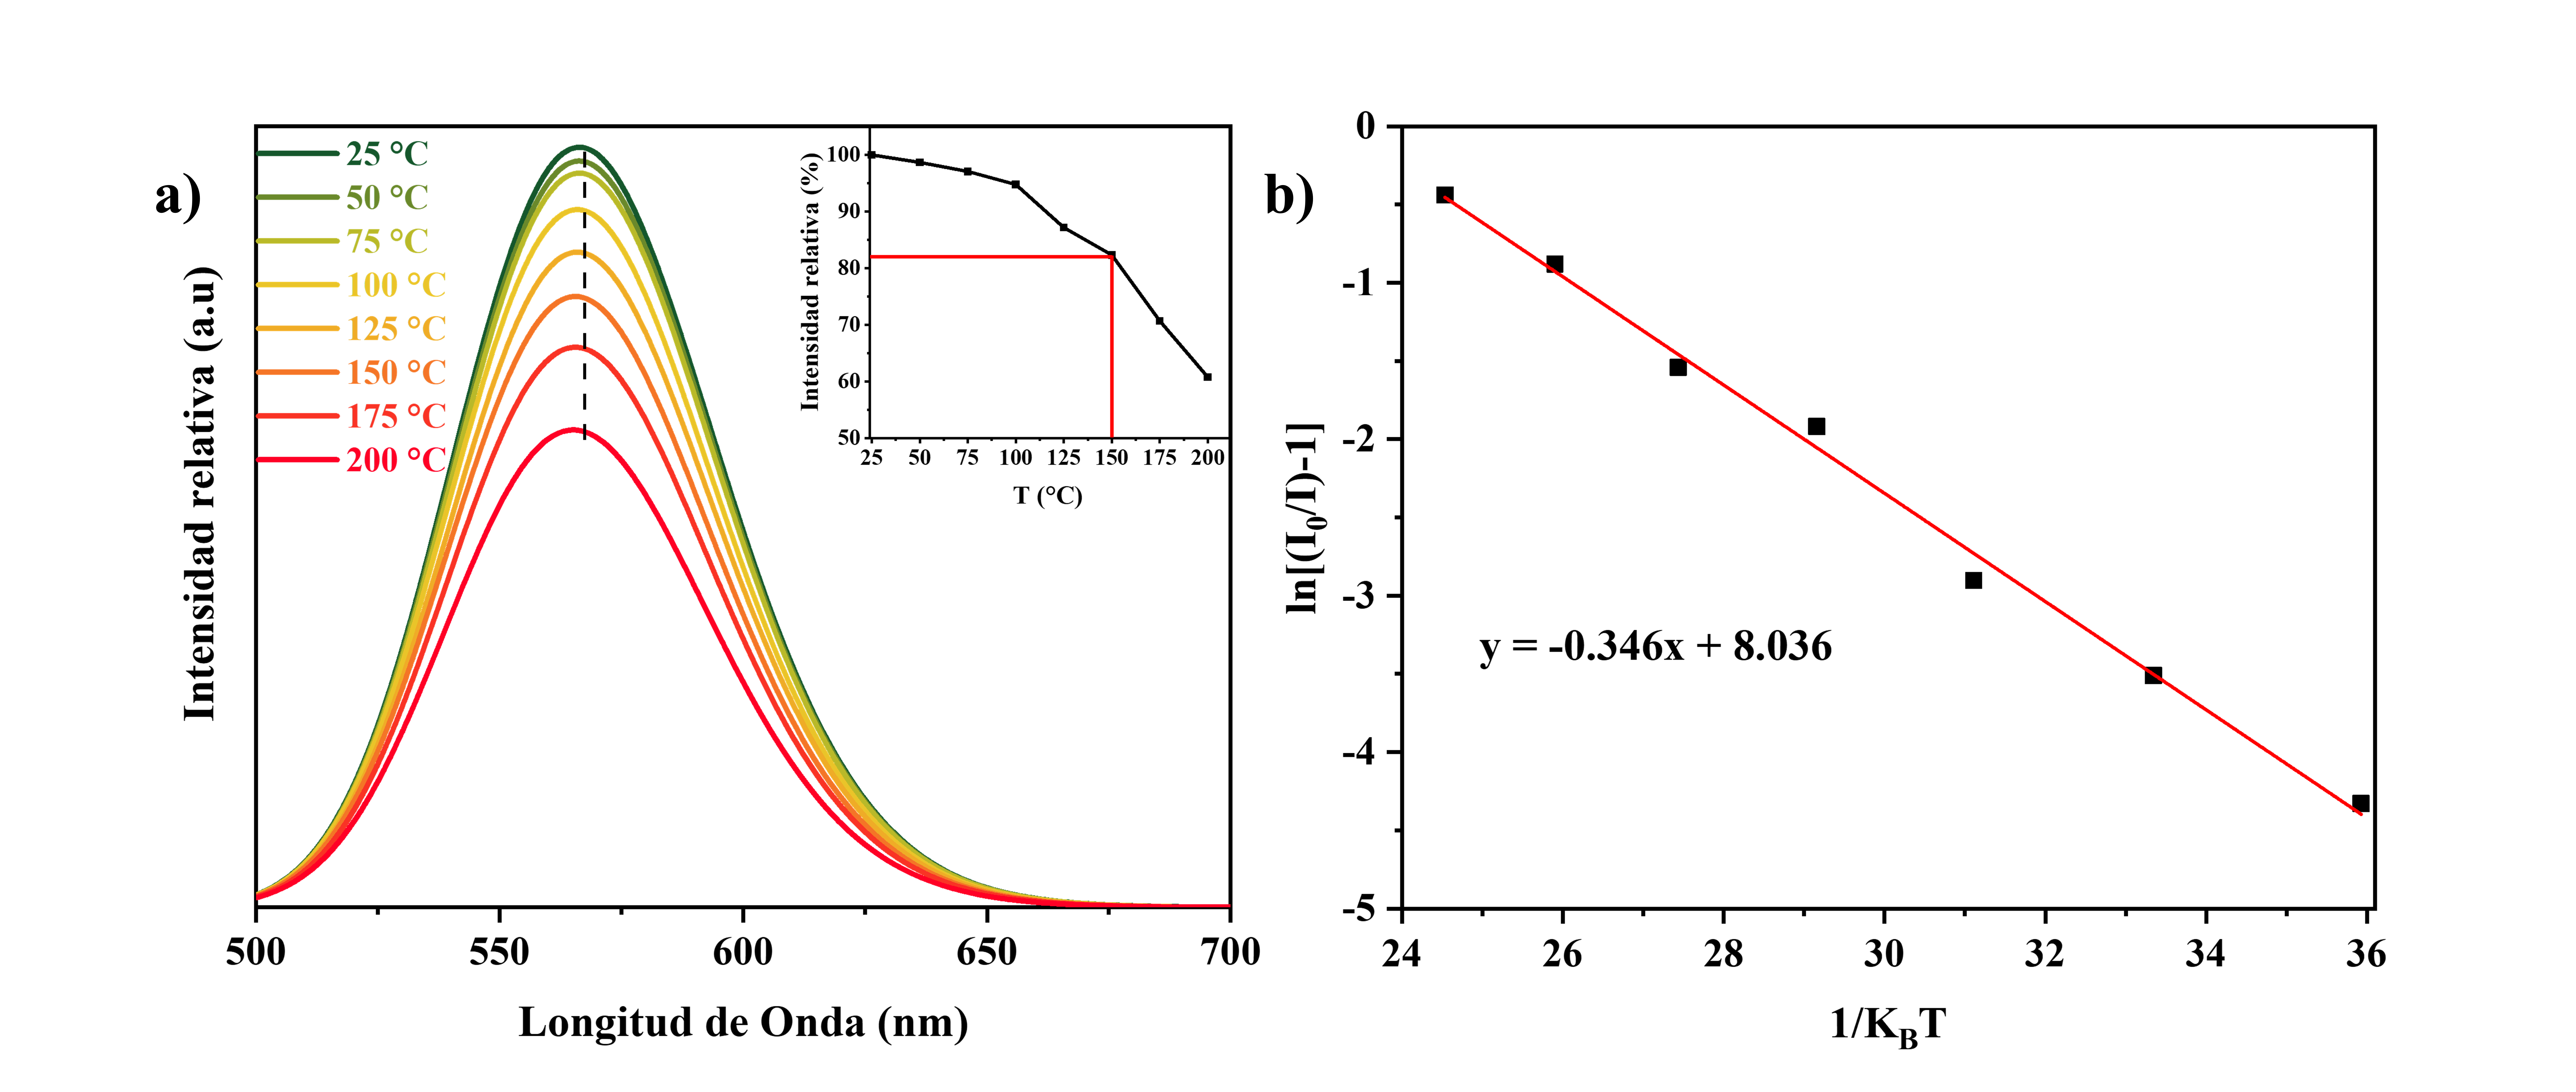
\includegraphics[width=\textwidth]{Kap4/fotoTemperatura.png}%
    \caption{Espectros de fotoluminiscencia en función de la temperatura para
    el fósforo \ce{Lu3Al_{1.5}Fe_{3.5}O12}:\ce{Ce^{3+}} (x = 3.5) bajo
    excitación
    de 436 nm, a) Intensidad de emisión relativa en función de la temperatura.
    b)
    Gráfica de $\ln[(I_{0}/I)-1]$ en función de $1/K_BT$}\label{fig:fotoTemp}
\end{figure}

La energía de activación ($\Delta E$) se calculó mediante la ecuación Arrhenius
(\ref{eqn:eq6}) \cite{Chen2015}.\\

\begin{equation}
    I=\frac{I_0}{1+A e^{-\Delta E/K_BT}}
    \label{eqn:eq6}
\end{equation}

Donde $I$ e $I_0$ indican la intensidad de emisión a la temperatura T y la
temperatura inicial (en escala absoluta), respectivamente. $A$ es una constante
y
$K_B$ es la constante de Boltzmann ($8.629×10^{-5} eV^{-1}$). $\Delta E$ se
determina mediante el
valor absoluto de la pendiente para la gráfica de $\ln [(I_0/I)-1] $ en función
a $1/K_{B}T$ (Figura \ref{fig:fotoTemp} b). El valor obtenido de $\Delta E$ fue
de $0.346 eV$, que es relativamente
alto y
muestra propiedades térmicas sobresalientes.\\